\documentclass[]{article}



\usepackage{graphicx,forloop,caption,subcaption,float,hyperref,arrayjob,listings,color,booktabs,mathtools}
\usepackage{pdfpages}
\usepackage{float}
\usepackage[margin=1.2in]{geometry}
\usepackage{amsmath}
\usepackage{amsthm}
\usepackage{multirow}
%vhdl code
\definecolor{dkgreen}{rgb}{0,0.6,0}
\definecolor{gray}{rgb}{0.5,0.5,0.5}
\definecolor{mauve}{rgb}{0.58,0,0.82}

\DeclareMathOperator*{\argmin}{\arg\!\min}
\newcommand{\rom}[1]{\uppercase\expandafter{\romannumeral#1}}

% declare theorem definitions
\newtheorem{thm}{Condition}

\lstset{frame=tb,
  language=VHDL,
  aboveskip=3mm,
  belowskip=3mm,
  showstringspaces=false,
  columns=flexible,
  basicstyle={\small\ttfamily},
  numbers=none,
  numberstyle=\tiny\color{gray},
  keywordstyle=\color{blue},
  commentstyle=\color{dkgreen},
  stringstyle=\color{mauve},
  breaklines=true,
  breakatwhitespace=true
  tabsize=3
}


%matlab code
\lstset{frame=tb,
  language=Matlab,
  aboveskip=3mm,
  belowskip=3mm,
  showstringspaces=false,
  columns=flexible,
  basicstyle={\small\ttfamily},
  numbers=none,
  numberstyle=\tiny\color{gray},
  keywordstyle=\color{blue},
  commentstyle=\color{dkgreen},
  stringstyle=\color{mauve},
  breaklines=true,
  breakatwhitespace=true
  tabsize=3
}


% Title Page
\title{UCLA\\EE230B\\Digital Communication Design Project\\Step 5 Report}
\author{Alican Salor 404271991 \\  \href{mailto:alicansalor@ucla.edu}{alicansalor@ucla.edu} \\ \\
Darren Reis 804359840 \\
\href{mailto:darrer.r.reis@gmail.com}{darren.r.reis@gmail.com} }


\begin{document}
\maketitle

\newpage
\tableofcontents

\newpage
\section{Background}
\label{sec:background}
This step of the project deals with the effect of Inter Symbol Interference (ISI), when residual signal from symbols meddles the level of subsequent symbols.  This has previously not been modeled in the system because we have been considering an ideal scenario.  In reality, transmission over a channel has to deal with the finite bandwidth of the medium.  Because of the bandlimiting, where the response of the system is 0 above a limiting frequency, the symbols will interfere with one another. To deal with the dispersion, the Zero-ISI condition [\ref{thm:zero}] must be met.  A number of techniques can be utilized to accomplish what effectively amounts to canceling out delayed versions of symbols:


 

\begin{itemize}
\item Use $C^{-1}\left(f\right)$ to undo the channel
\item Use precoding
\item Use Nyquist's Pulse-Shaping Criterion and MLSE
\item Use an Equalizer
\end{itemize}
For this project, we use an Equalizer to handle the ISI.  \\

\begin{thm}
\label{thm:zero}
Zero-ISI:
$$x\left(nT\right) = \left\{
\begin{array}{1 1}
1 & \quad n=0 \\
0 & \quad \text{else}
\end{array} \right.$$
\end{thm}

\begin{figure}[H]
\centering
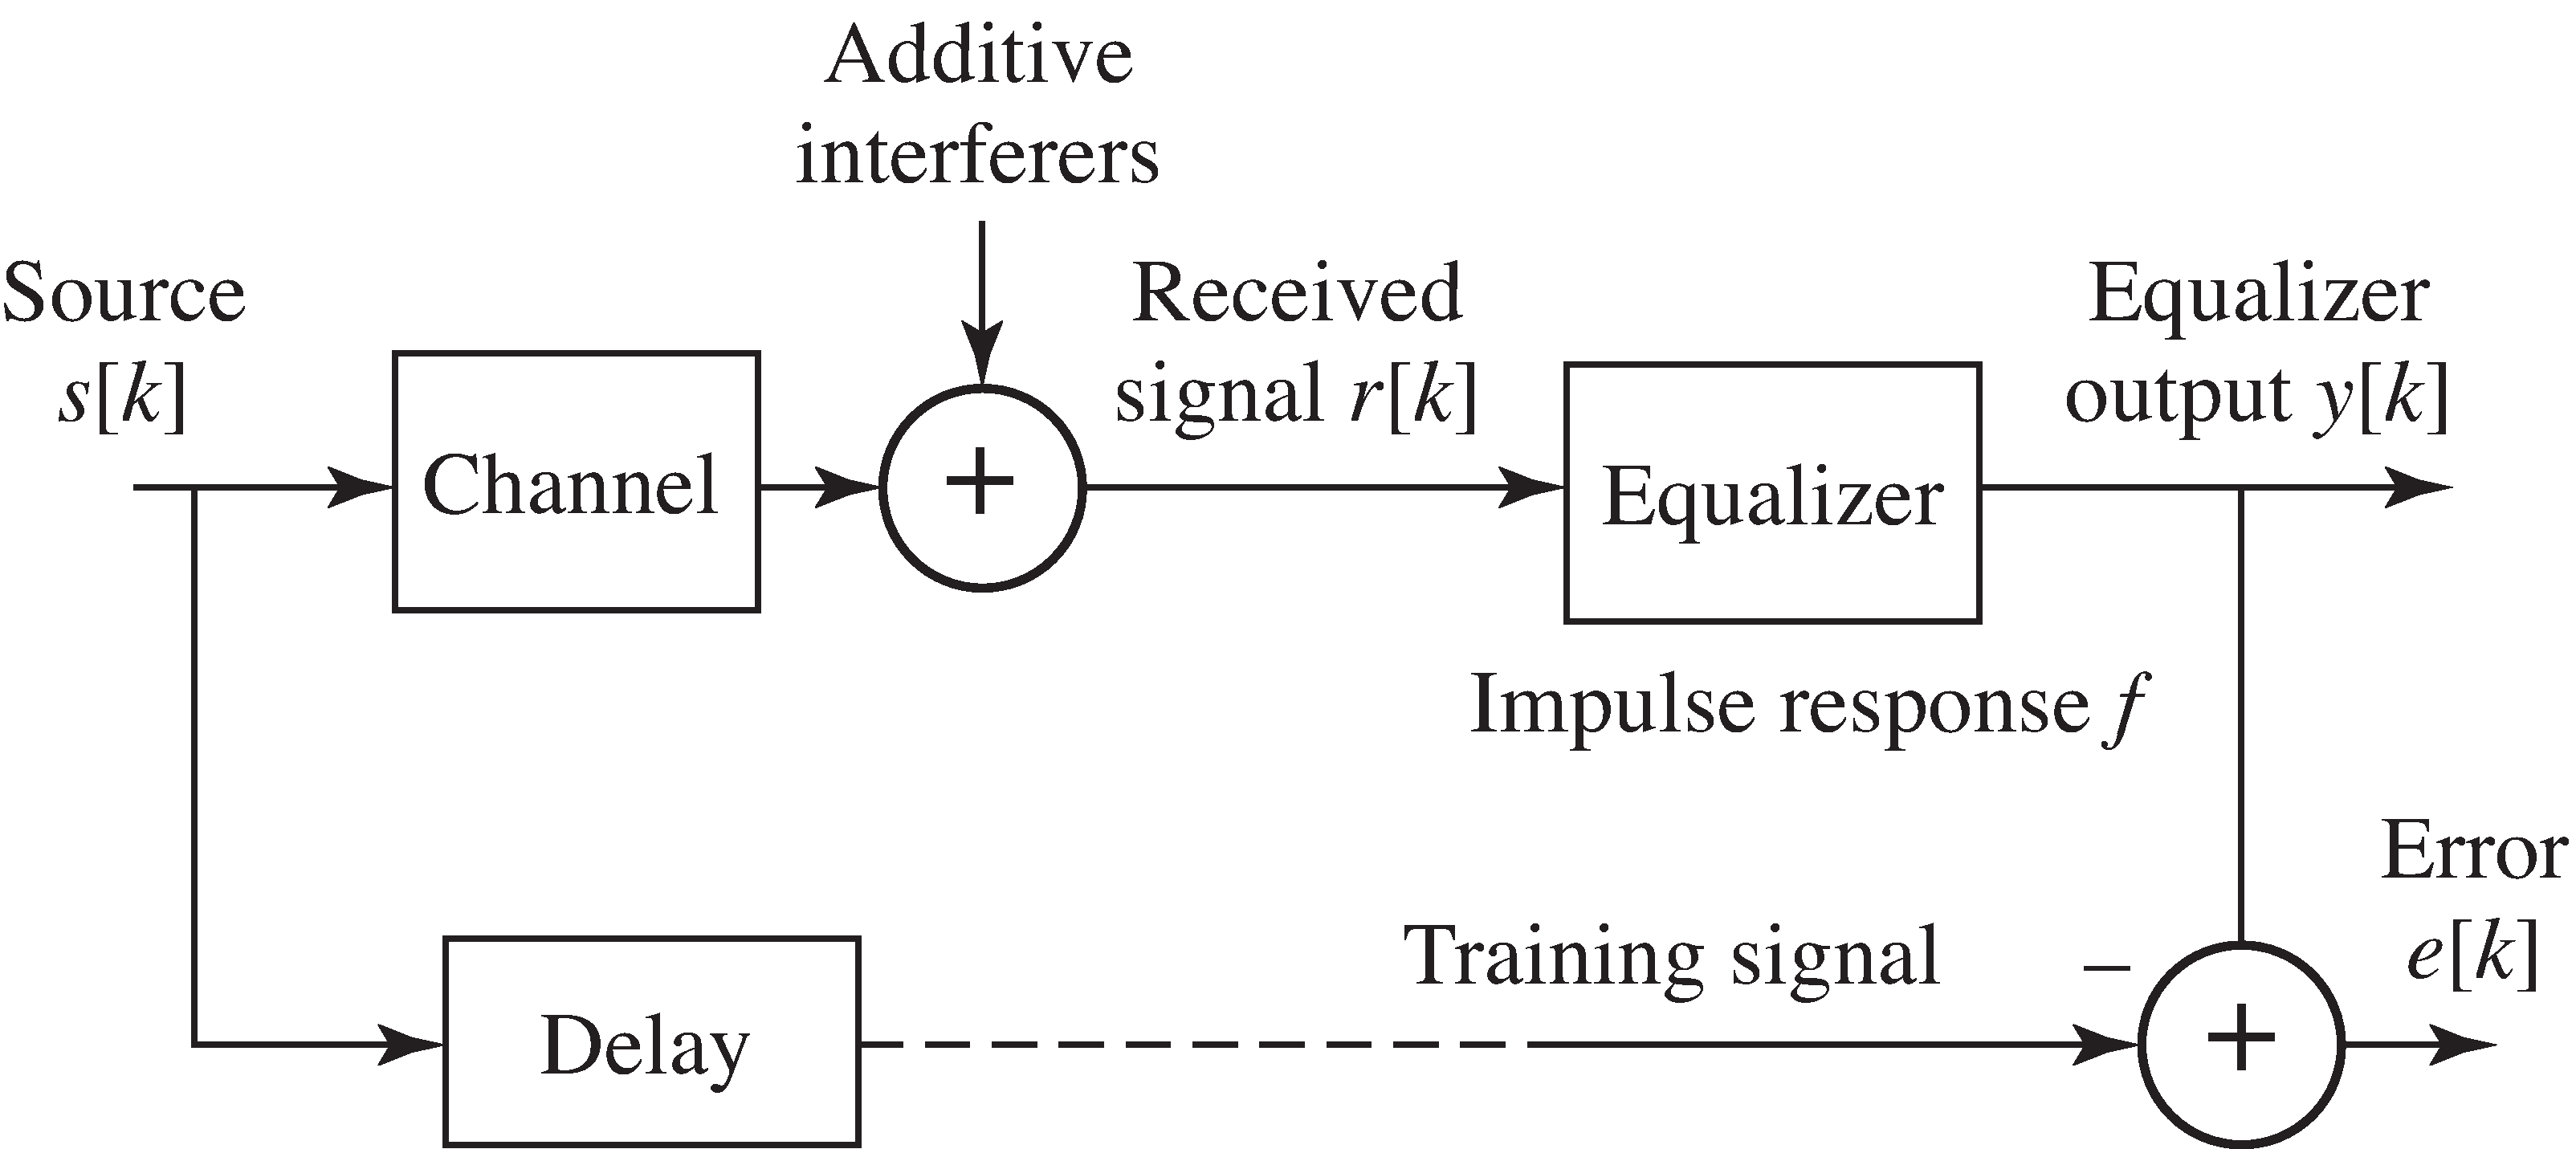
\includegraphics[width=\textwidth]{equalizer.png}
\caption{Generic Equalizer Filter to zero out the ISI\label{fig:equalizer}}
\end{figure}

An equalizer is a filter that zeros out the ISI in the end-to-end system.  It can be preset to handle the channel, or can adapt to the time-varying nature of a channel.  In the latter case, the equalizer parameter are adjusted on the fly by periodic transmission of a known sequence to re-estimate the channel.  In either case, the equalizer is a filter whose frequency response counteracts the system model such that Condition~\ref{thm:zero} is met.  

Considering this system, where Table~\ref{tab:filtersummary} describes the variables, we can determine the channel response first by 

\begin{table}[H]
\begin{center}
\begin{tabular}{|c|c|c|c|}
\hline Variable & Meaning & Dimensions \\
\hline \hline
$\vec{s}$ & Source & mx1 \\ \hline
$\vec{r}$ & Received Signal & mx1 \\ \hline
$R$ & Channel Response Matrix & pxn \\ \hline
$\vec{f}$ & Tap Line / Impulse Response & nx1 \\ \hline
$\vec{y}$ & Equalizer Output & mx1  \\ \hline
 $\vec{e}$ & Training Error & mx1 \\ \hline
\end{tabular}
\caption{Summary of Signals and Variables} \label{tab:filtersummary}
\end{center}
\end{table}

\begin{table}[H]
\begin{center}
\begin{tabular}{|c|c|}
\hline Parameter & Meaning \\
\hline \hline
$m$ & Signal Length \\ \hline
$n$ & Filter Order \\ \hline
$p$ & Training Sequence Length \\ \hline
\end{tabular}
\caption{Summary of Parameters} \label{tab:Paramsummary}
\end{center}
\end{table}

The direct form FIR is shown in Figure~\ref{fig:tap}.  The filter transfer function can be seen in Equation~\ref{eq:equalizer}.  The objective for this filter is to counter the system channel.  For our case, we did a one-shot channel estimation and used the results over the entirety of the experiment.  \\


\begin{equation}
\label{eq:equalizer}
y\left[k\right] = \sum_{j=0}^n f_jr\left[k-j\right]
\end{equation}

To do channel estimation, we sent a known sequence through the system and BLAH BLAH. \\

The FIR form of the equalizer can then be written as Equation~\ref{eq:equalizerVector} and Equation~\ref{eq:equalizerMatrix}.  The compact form of this relation uses a matrix equation where the filter is expressed as a Toeplitz matrix.  This neat fact allows us to use the power of linear algebra to solve for the zero forcing channel.  
  
\begin{equation}
\label{eq:equalizerVector}
\left[ \begin{array}{c}
 y \left[n+1\right] \\
 y \left[n+2\right] \\
 y \left[n+3\right] \\
\vdots  \\
y\left[ p \right] \end{array} \right] = 
\begin{bmatrix} 
r \left[ n+1\right]  & r[n] \cdots & r\left[ 1 \right] \\ 
r \left[ n+2\right]  & r[n+1] \cdots & r\left[ 2 \right] \\ 
r \left[ n+2\right]  & r[n+2] \cdots & r\left[ 3 \right] \\ 
\vdots & \vdots & & \vdots \\
r \left[p \right] & r\left[ p-1 \right] & \cdots r\left[ p-n \right]
end{bmatrix} \left[ \begin{array}{c} f_0 \\ f_1 \\ f_2 \\ \vdots \\ f_n \right]
\end{equation}
\begin{equation}
\label{eq:equalizerMatrix}
\vec{y} = R\vec{f}
\end{equation}
What we want is to optimally force the channel to zero for all other symbols than the present one.  As an aside, because there is delay in the system, the intuitive sense of causality is blurred.  We can define a cost function, a metric to minimize, as in Equation~\

\begin{equation}
\label{eq:cost}
J(


Using the Penrose Psuedo Inverse, Equation~



\begin{equation}
\label{eq:mmse}

\end{equation}


\begin{figure}[H]
\centering
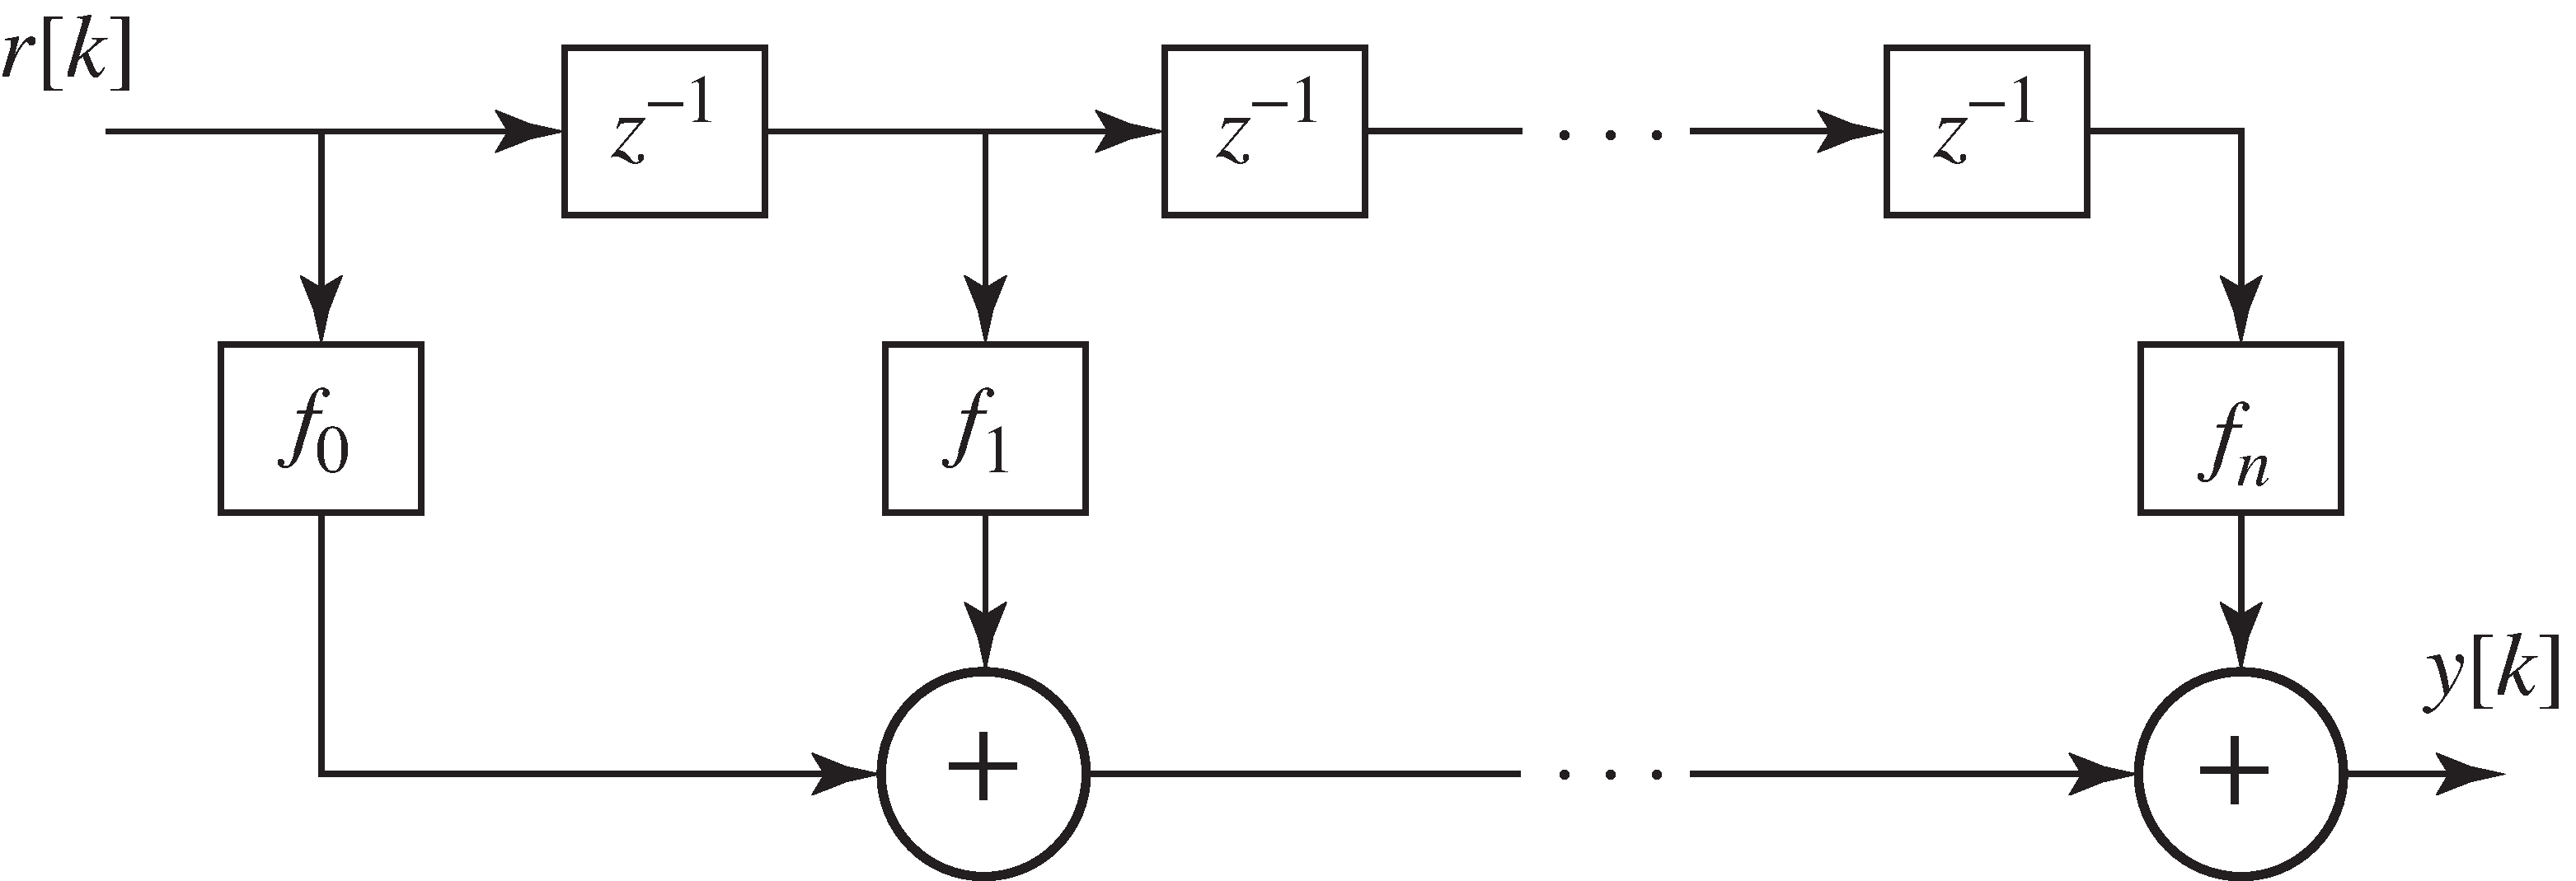
\includegraphics[width=\textwidth]{tapEqualizer.png}
\caption{Tapped Delay Line Represenation\label{fig:tap}}
\end{figure}

\newpage
\section{System}
\label{sec:system}
The system simulation model is shown in Figure~\ref{fig:step4}.  

\begin{figure}[H]
\centering
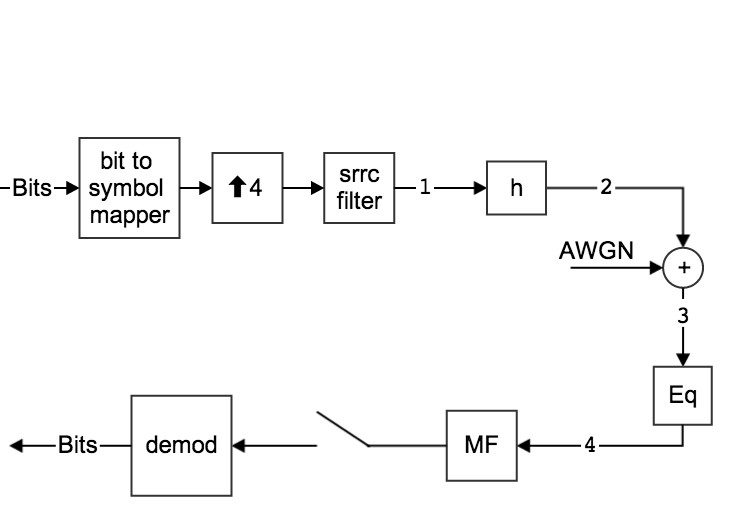
\includegraphics[width=\textwidth]{step5.png}
\caption{Block Diagram of Step 5 system setup\label{fig:step5}}
\end{figure}

As from Step 1, randomly generated bits [Appendix~\ref{app:random_bit_generator}] are converted into symbols [\ref{app:bittosym}] and then upsampled by adding in zeros [\ref{app:impulse_train}].  The result is then is run through a Square Root Raised Cosine (SRRC) pulse shape filter [\ref{app:sqrt_raised_cosine}].  This shaping improves the resistance of the sequence to intersymbol interference (ISI).  The output of this filter is fed into a Digital-to-Analog Converter (DAC).  A DAC takes the digital samples and zero-order holds them at a constant voltage, creating an analog signal [Appendix~\ref{app:da},~\ref{app:zero}]. After the digitizer, a reconstruction filter (also called an anti-aliasing filter) bandlimits the analog waveform output from the DAC.  The high frequency content contained in the stair-case digital signal is undesirable since it can create aliasing of wrongfully high frequency waves. To avoid this, the Low Pass Filter is used for the reconstruction.  Ours is modeled as a Butterworth filter, or a maximally flat magnitude filter.  The aim of the filter is to have uniformly flat passband frequency response and roll to zero in the stopband.  As with all filters, the cutoff frequency parameter sets the bands and the order of the filter determines the roll-off of the frequency response in the stopband.  We used a fourth order Butterworth so that the roll-off was $80 \mathtt{\frac{dB}{dec}}$.  We set the cutoff frequency approx. to $\frac{\pi}{20}$ $\mathtt{Hz}$ at the TX part. The interior workings of the filter are not pertinent to this project, so the code in Appendix~\ref{app:butterworth} uses built-in MATLAB functions.  \\



The end of the simulation model is identical to the process in Step 1: a matched filter to the SRRC picks out the symbols from the noisy received signal.  Afterwards, a sampler recovers [Appendix~\ref{app:sampler}] the symbols before a demodulator converts the symbols back into bits [\ref{app:dblocks}].  


\section{Step 4 Results}
\label{sec:results}
In the following sections, the results of the simulations of the different modulation schemes are shown.  For each SER plot, the corresponding results from Step 1 are presented alongside.  The results are interpreted afterwards in the conclusion section.

\newpage
\subsection{Probability Error Rate Comparison}
\label{sec:compare}

\newpage
\subsection{Constellation Comparison}
\label{sec:constCompare}

\newpage
\section{Conclusion}
\label{sec:conc}

BLAH

\appendix
\newpage
\bibliographystyle{plain}
\bibliography{step4}
\newpage
%% the \\ insures the section title is centered below the phrase: Appendix B
%\section{Project Assignment}
%\label{app:assign}
%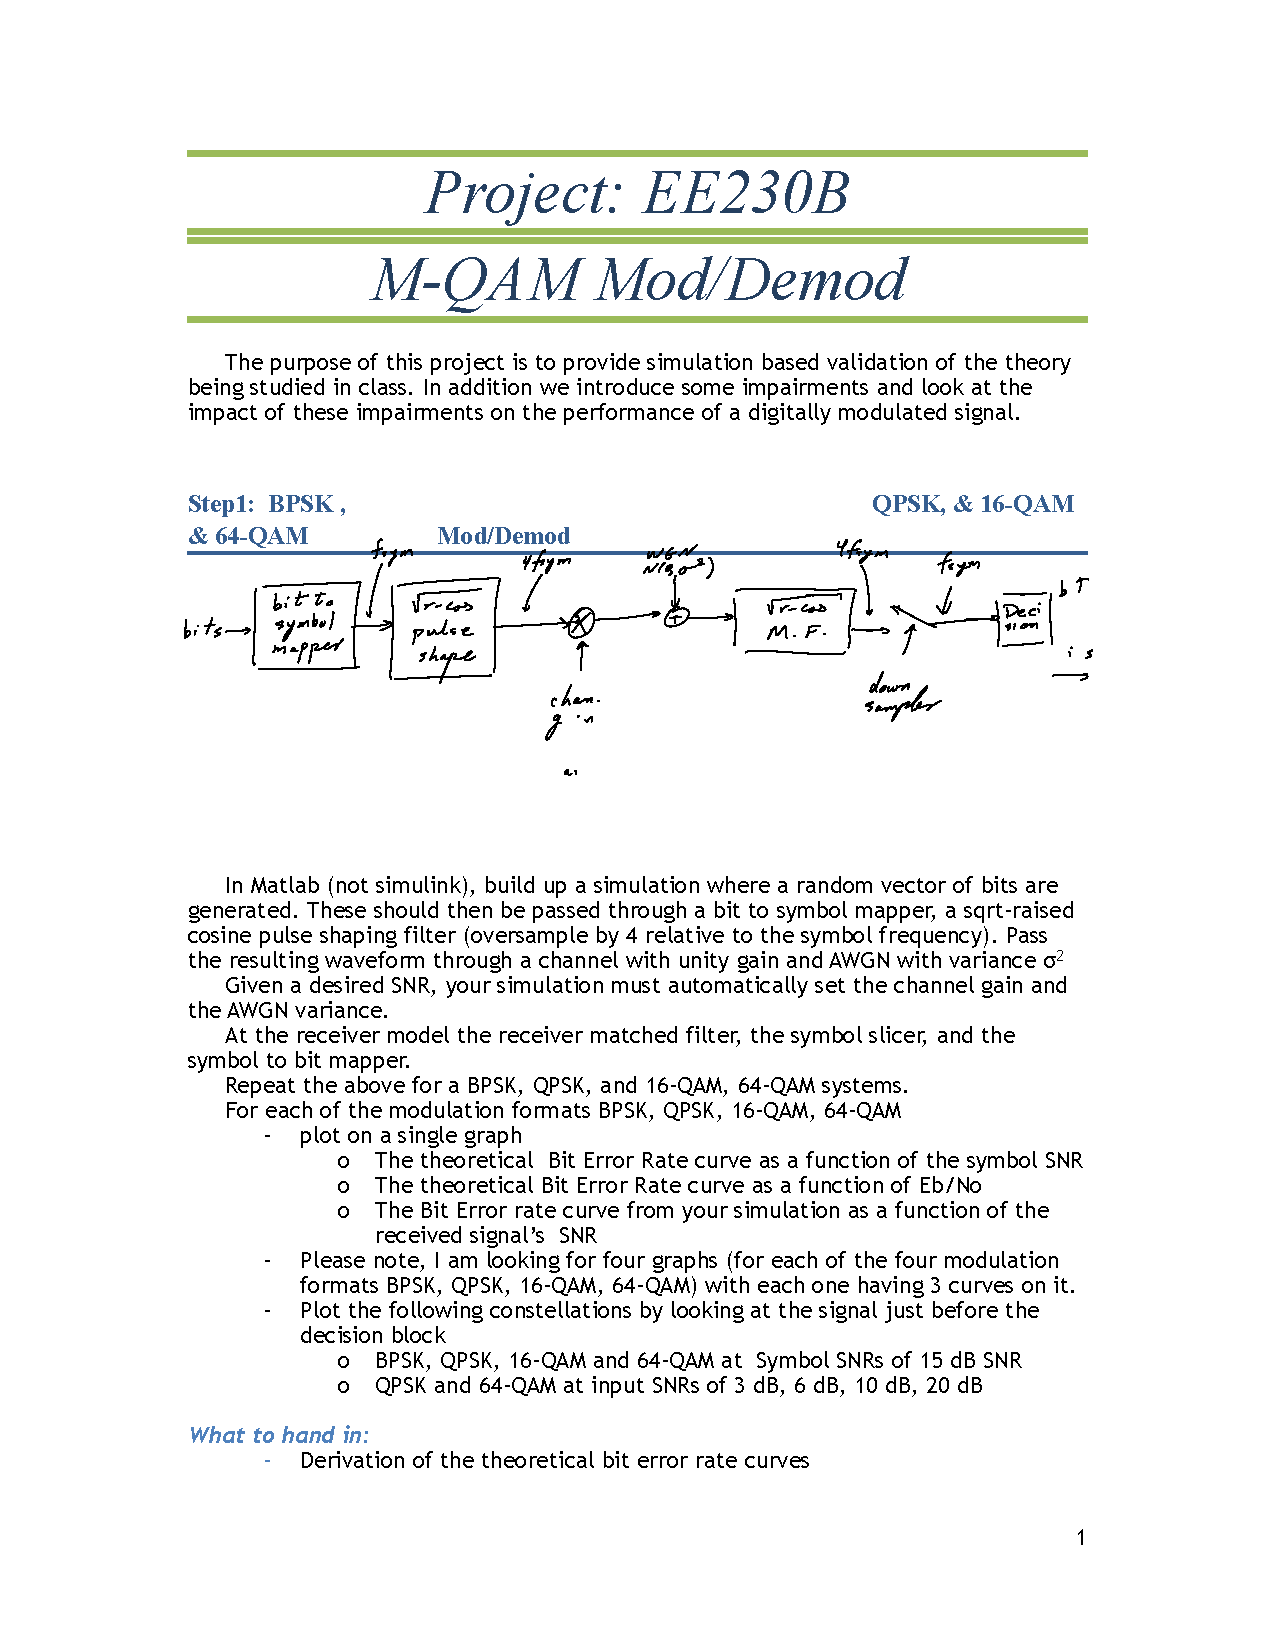
\includepdf[pages={1-5}]{project_overview.pdf}
%\cleardoublepage
%\newpage

\section{Random Bit Sequence Generator}
\label{app:random_bit_generator}
\lstinputlisting{random_bit_generator.m}

\section{Bit to Symbol Mapper}
\label{app:bittosym}
\subsection{BPSK Modulation}
\label{app:bpsk_mod}
\lstinputlisting{bpsk_mod.m}

\subsection{QPSK Modulation}
\label{app:qpsk_mod}
\lstinputlisting{qpsk_mod.m}

\section{Up Sampler}
\label{app:impulse_train}
\lstinputlisting{impulse_train.m}

\section{Square Root Raised Cosine Filter}
\label{app:sqrt_raised_cosine}
\lstinputlisting{sqrt_raised_cosine.m}

\section{Additive Gaussian White Noise Channel}
\label{app:awgn_channel}
\lstinputlisting{awgn_complex_channel.m}

\section{Sampler}
\label{app:sampler}
\lstinputlisting{sampler.m}

\section{Decision Block}
\label{app:dblocks}
\subsection{BPSK Demodulation}
\label{app:bpsk_demod}
\lstinputlisting{bpsk_demod.m}

\subsection{QPSK Demodulation}
\label{app:qpsk_demod}
\lstinputlisting{qpsk_demod.m}

\subsection{16-QAM Demodulation}
\label{app:16qam_demod}
\lstinputlisting{qam_16_demod.m}

\subsection{64-QAM Demodulation}
\label{app:64qam_demod}
\lstinputlisting{qam_64_demod.m}

\section{Butterworth Filter}
\label{app:butterworth}
\lstinputlisting{ButterworthFilter.m}

\section{Conversion}
\label{app:convert}
\subsection{Analog-to-Digital Converter}
\label{app:ad}
\lstinputlisting{AD_conv.m}
\subsection{Digital-to-Analog Converter}
\label{app:da}
\lstinputlisting{DA_conv.m}

\subsection{Zero Hold}
\label{app:zero}
\subsection{Decimation}
\lstinputlisting{ZeroHoldDecimation.m}
\subsection{Interpolation}
\lstinputlisting{ZeroHoldInterpolation.m}

\section{Sensitivity}
\label{app:sensitivity}

\subsection{Sampling Delay Analysis}
\label{app:delay}
\lstinputlisting{sensitivityDelay.m}

\subsection{TX Filter $f_c$ Shifting Analysis}
\label{app:freqTX}
\lstinputlisting{sensitivityFreqTX.m}

\subsection{RX Filter $f_c$ Shifting Analysis}
\label{app:freqRX}
\lstinputlisting{sensitivityFreqRX.m}

\section{Simulations}
\subsection{BPSK Simulation}
\lstinputlisting{step4_sim_bpsk.m}

\subsection{QPSK Simulation}
\lstinputlisting{step4_sim_qpsk.m}

\subsection{16-QAM Simulation}
\lstinputlisting{step4_sim_QAM16.m}

\subsection{64-QAM Simulation}
\lstinputlisting{step4_sim_QAM64.m}

\end{document}
